\documentclass{standalone}
\usepackage{pgfplots}

\begin{document}

\tikzset{every picture/.style={line width=0.75pt}} %set default line width to 0.75pt        

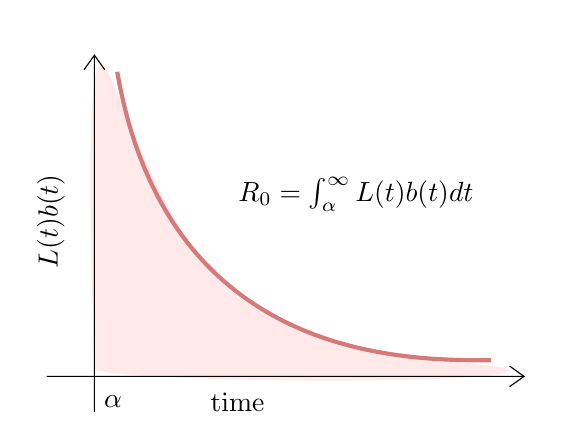
\begin{tikzpicture}[x=0.75pt,y=0.75pt,yscale=-1,xscale=1]
%uncomment if require: \path (0,219); %set diagram left start at 0, and has height of 219

%Shape: Polygon Curved [id:ds584900939003939] 
\draw  [draw opacity=0][fill={rgb, 255:red, 255; green, 233; blue, 233 }  ,fill opacity=1 ] (55,31) .. controls (61,10) and (78,104) .. (123,139) .. controls (168,174) and (267,170) .. (252,176) .. controls (237,182) and (54,180.46) .. (54,173.73) .. controls (54,167) and (49,52) .. (55,31) -- cycle ;
%Shape: Axis 2D [id:dp5118438497491022] 
\draw  (31,177.73) -- (261,177.73)(54,23) -- (54,194.92) (254,172.73) -- (261,177.73) -- (254,182.73) (49,30) -- (54,23) -- (59,30)  ;
%Curve Lines [id:da895630980425018] 
\draw [color={rgb, 255:red, 214; green, 121; blue, 121 }  ,draw opacity=1 ][line width=1.5]    (65,31) .. controls (89,170) and (203,170) .. (245,170) ;



% Text Node
% \draw (721,21) node   {$0$};
% Text Node
% \draw (701,71) node   {$0$};
% Text Node
\draw (33,103) node [rotate=-270.08] [align=left] {$L(t)b(t)$};
% Text Node
\draw (123,190) node  [align=left] {time};
\draw (63,190) node  [align=left] {$\alpha$};

\draw (180,90) node [align=left] {$R_0 = \int_{\alpha}^{\infty}L(t)b(t) dt$};



\end{tikzpicture}
\end{document}